

This appendix contains the \textquote{developer report}, a document written up after development evaluating the experience of developing the prototype, alongside discussion of more subjective elements of the evaluation.

\par\noindent\rule{\textwidth}{0.25mm}

Within the development period allocated (including the 2 week overflow used), the prototype core systems were developed, however development was not able to proceed beyond this point. Development itself was enjoyable, but slow. Feature creep did not occur, thus this extended development period was exclusively a consequence of the core systems, namely CatCode.

\section{Engine Choice}

With the exception of CatCode (more in \autoref{sec:devRep/catCode}), Godot and GDscript were a good engine and programming language for this project. The limitations of the engine/language did not cause any issues and their emphasis on simpler design and nodes aided with the speed of development required for the prototype. As well as this, the graphical tools packaged with the engine aided with level design and debugging, including one instance when a memory leak occurred within catCode interpretation (shown in \autoref{fig:memoryLeak}).

\begin{figure}
    \centering
    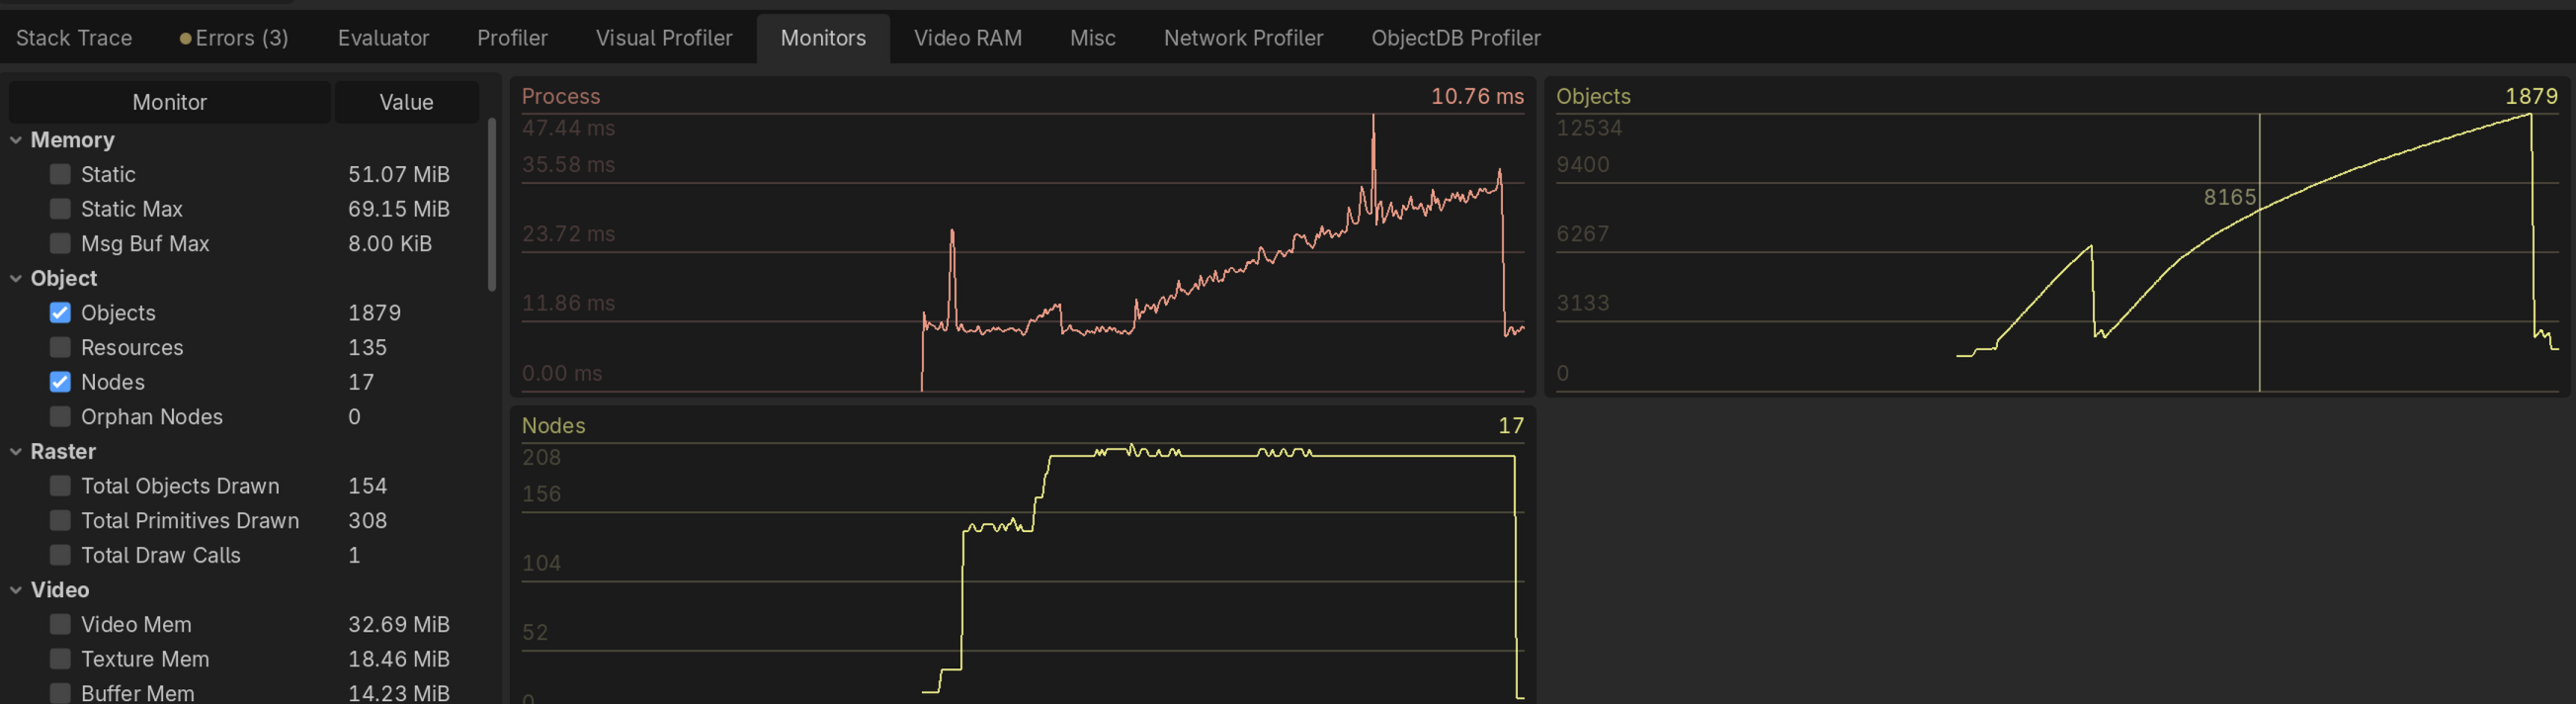
\includegraphics[width=1\linewidth]{AC/memoryLeak.png}
    \caption{Godot object tracker during a memory leak}
    \label{fig:memoryLeak}
\end{figure}

\section{Development Time}

It was originally expected that 6 weeks would have been sufficient time to develop a prototype game with a few prototype levels and the implemented core systems. This was based on previous expedience participating in game jams with stricter time limits.

Due to the complex nature of this game, incorporating a basic internal programming language for the player to use, it was expected that the core systems would take 1.5 to 3 weeks, not the 8 weeks it ended up being. During our research, we were not able to find a comparable project, with the transparency that would provide the data required to estimate the required development period. Therefore, it is reasonable that this could not have been foreseen.

\section{Developing CatCode}\label{sec:devRep/catCode}

As mentioned before, CatCode took significantly longer to develop than anticipated and single-handed caused the development time to overrun. This was because the entire system was more complicated to implement than initially anticipated. It could be argued that spending more time to undergo a more rigorous design process could have uncovered this.

The godot wiki argues that exceptions are not needed for games \citep{GodotExceptions}, which is usually true, however CatCode ended up being far closer to a programming language than a system in a game in its final form. As a result of this, a custom error handeling system needed to be developed. This significantly slowed down development, and was potentially not needed once Graphical CatCode was implemented.

Another common function of object orientated programming languages whose absence was noticed were access modifiers. Due to these not being used, one had to keep track of which variables were mean to be used and which were not by scripts external to the node. In a similar vein, the absence of interfaces (and multiple inheritance of interfaces) in GDscript further complicated development and meant that we could not follow the objected orientated best practice of \textquote{program[ing] to interfaces not to implementation} \citep{oop-ptinti}.

The lack of exception handling, access requirements and interfaces could have been solved by using C\# rather than GDscript as Godot has compatibility for this at the cost of the ability to export to web platforms \citep{GodotCSharp}. The main issue that remained that would not be able to be fixed is the inconsistent used of signals and functions, and reused variable names in different nodes/contexts (repeated use of \texttt{parent} for example), however neither of these would be fixable without going back to the drawing boards or spednding a significant amount of time that was not available refactoring existing systems.

In spite of the flaws, CatCode was a good system that performs its function adequately and without significant resource usage. As well as this, evidence points towards the high time commitment to develop would be contained to creating the foundations of the system. This was tested through the implementation of the blocks \texttt{and}, \texttt{or}, \texttt{not} and \texttt{can\_strike()} which was done within one day, taking around 4 hours of work.

\section{Puzzle and Level Design}

Creating levels was easy using the built-in Godot editor, using the \textit{tilemap} node. Setting instruction sets and auto-controllers was also simple through dragging packed scenes onto to CatBot, either as a child of \textit{catCodeManager} for logic blocks, or as a child of CatBot for auto-controllers.

Puzzle design, however, was a bit more complicated. Certain elements of programming were more intuitive to design levels around then others. For example, the platformer format was well suited to selection due to many elements falling into a pattern of \textquote{if button pressed: jump}, whereas iterative elements were harder to incorporate due to not fitting as naturally into a function that is executed every frame. Regardless of elements, there would be a risk that puzzles could become repetitive unless they branch out beyond recreating typical platforming systems for CatBot.

\section{Conclusions}

\begin{enumerate}
        \item The Godot engine was the right choice for many reasons, but also had numerous drawbacks.
        \item 8 weeks were not sufficient for developing this game.
        \item Exception handling, whilst not always helpful for game development, would have made CatCode easier to develop.
        \item Stronger typing, as well as public and private methods and variables, would have also made development easier.
        \item Due to lack of well-documented similar systems, there was no reasonable way to foresee any of the issues that occurred.
        \item Once the foundations were finished (approximately 3 days before the feature freeze) development was far quicker.
        \item The platformer approach lends itself well to selection (if etc.) based puzzles, however it struggled to incorporate iteration. Plus, Puzzles may quickly become repetitive.
        \item In spite of the drawbacks, development was still enjoyable.
    \end{enumerate}

